\documentclass[12pt]{letter}
\usepackage{amsmath}
\usepackage{graphicx}
\usepackage{wrapfig}
\pagestyle{empty}
\usepackage{textcomp}		
\usepackage{setspace}

\begin{document}
%Begin
%Language English
%Source Calgary Junior High School Mathematics Contest
%Title Part A 1998
%Question 7
%Subject algebra
%Category manipulations
%Type SA
%Answer C
%Creator Duncan Long
%Rdifficulty 21
%Qtext
\footnotesize{Source: Calgary Junior High School Mathematics Contest}\\ \\

\begin{wrapfigure}[6]{r}{55mm}
  \begin{center}
    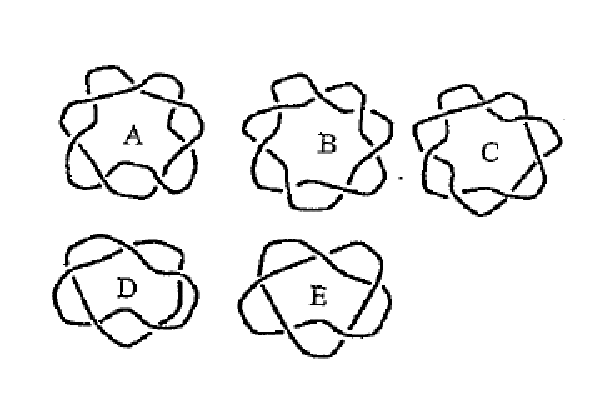
\includegraphics[scale=0.75]{CAJA98-07fig.eps}
  \end{center}
\end{wrapfigure}
\large
The following five curves represent loops of string, with crossings indicating where one piece of string passes over another piece. Which one of the five strings can be unravelled into a loop with no knot in it?	 \\ \\ \\

%Ftext
\textbf{The correct answer is C} 

\begin{wrapfigure}[6]{r}{55mm}
  \begin{center}
    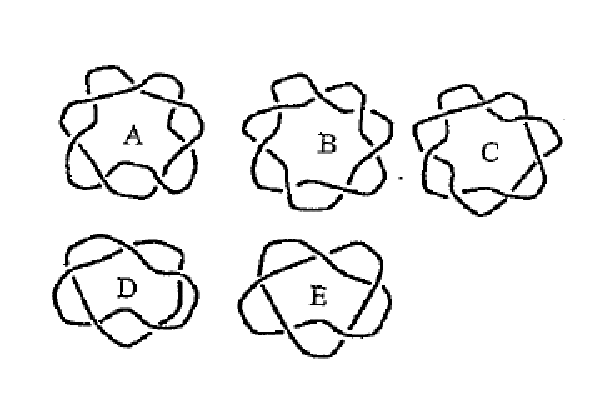
\includegraphics[scale=0.75]{CAJA98-07fig.eps}
  \end{center}
\end{wrapfigure}
String C is the only figure which can be unravelled into a simple loop. 
\pagebreak
%End
\end{document}